\documentclass[10pt, compress]{beamer}
% Light colors
% Frame with section title at the beginning of each section
\usepackage[light,sectionframe]{../beamerthemesolarized} % if the .sty file is in ../
%\usetheme[light,sectionframe]{solarized} % if the theme is globally installed

\usepackage[english]{babel}
\usepackage{graphicx} % Graphics
\usepackage{subfig}   % Juxtapose figures


\title{Investigation on the theory of the Brownian Motion}
\subtitle{A short overview}
\date{\today}
\author{Albert Einstein, Ph.D.}
\institute{Swiss Federal Institute of Technology in Zurich}

\begin{document}

\maketitle

\begin{frame}{Introduction}{Goal of this study}
\begin{block}{}
\vspace{-0.2cm}
We aim at building a new theory for \textcolor{solarizedYellow}{random movement} of particles
\begin{itemize}
\item Bla bla
\item Bla bla
\item Bla bla
\end{itemize}
because \textbf{bla bla}.
\end{block}
\end{frame}

\begin{frame}{Contents}
\tableofcontents
\end{frame}

% First section
\section{On the movement of small particles in a stationnary liquid}

\subsection{System description}

\begin{frame}{System description}{Particles in a stationnary liquid}
\begin{columns}
\begin{column}{0.5\textwidth}
\begin{figure}
\hspace*{-0.75 cm}
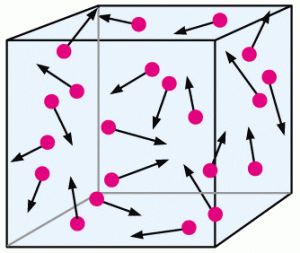
\includegraphics[width=5.5cm]{particles.png}
\caption{System representation}
\end{figure}
\end{column}

\begin{column}{0.5\textwidth}
\begin{itemize}
    \item Elementary particles
    \item Thermal agitation
    \item Random collisions
\end{itemize}
\end{column}

\end{columns}
\end{frame}


\subsection{Movement equations}
\subsection{New framework for movement description}

% Second section
\section{On the theory of Brownian Motion}

\subsection{Definitions}
\subsection{Main result}

\begin{frame}{Einstein's equations}{Particles in a stationnary liquid}
\begin{block}{Main result}
For particles in a stationnary liquid, we have:
$$
< (\Delta x)^2 > ~=~ \frac{RT}{N} \frac{1}{3 \pi \mu a} \tau
$$

\end{block}
\end{frame}

\subsection{Consequences and perspectives}


\begin{frame}{Some interesting perspectives}{Few insights}
I think that 
\begin{itemize}
    \item Bla bla bla
    \item Bla \textcolor{solarizedYellow}{bla bla}
    \item Bla bla bla
    \item Bla bla bla
\end{itemize}
has to be further examined...
\end{frame}
\end{document}
